\section{DC Sweep Simulation}
The schematic in the first exersice with \textbf{R1 = 1k} is re-used in this exercise. However, a DC-Sweep simulation mode is performed with V1 is varied from 0V to 5V (0.1V for the step), as follows:

\begin{figure}[!htp]
    \centering
    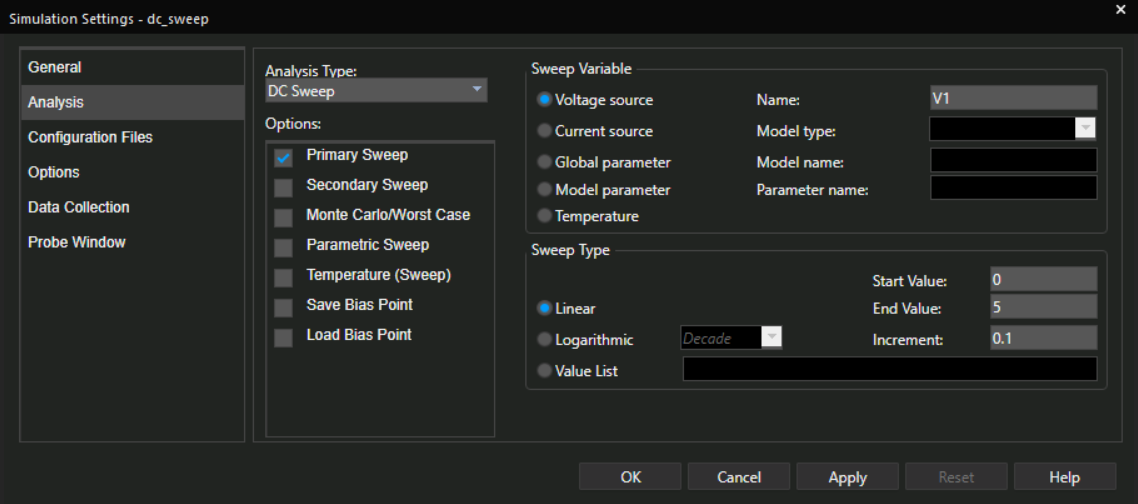
\includegraphics[width=0.8\linewidth]{graphics/ex2/f1.PNG}
    \caption{\textit{DC-Sweep profile for simulation}}
\end{figure}

Run the simulation and trace for the current $I_C$ according to the value of $V_1$. Capture your screen and plot it in the report. Please increase the width of the curve.

\begin{figure}[!htbp]
    \centering
    \textbf{\textit{Your image goes here:}}\\
    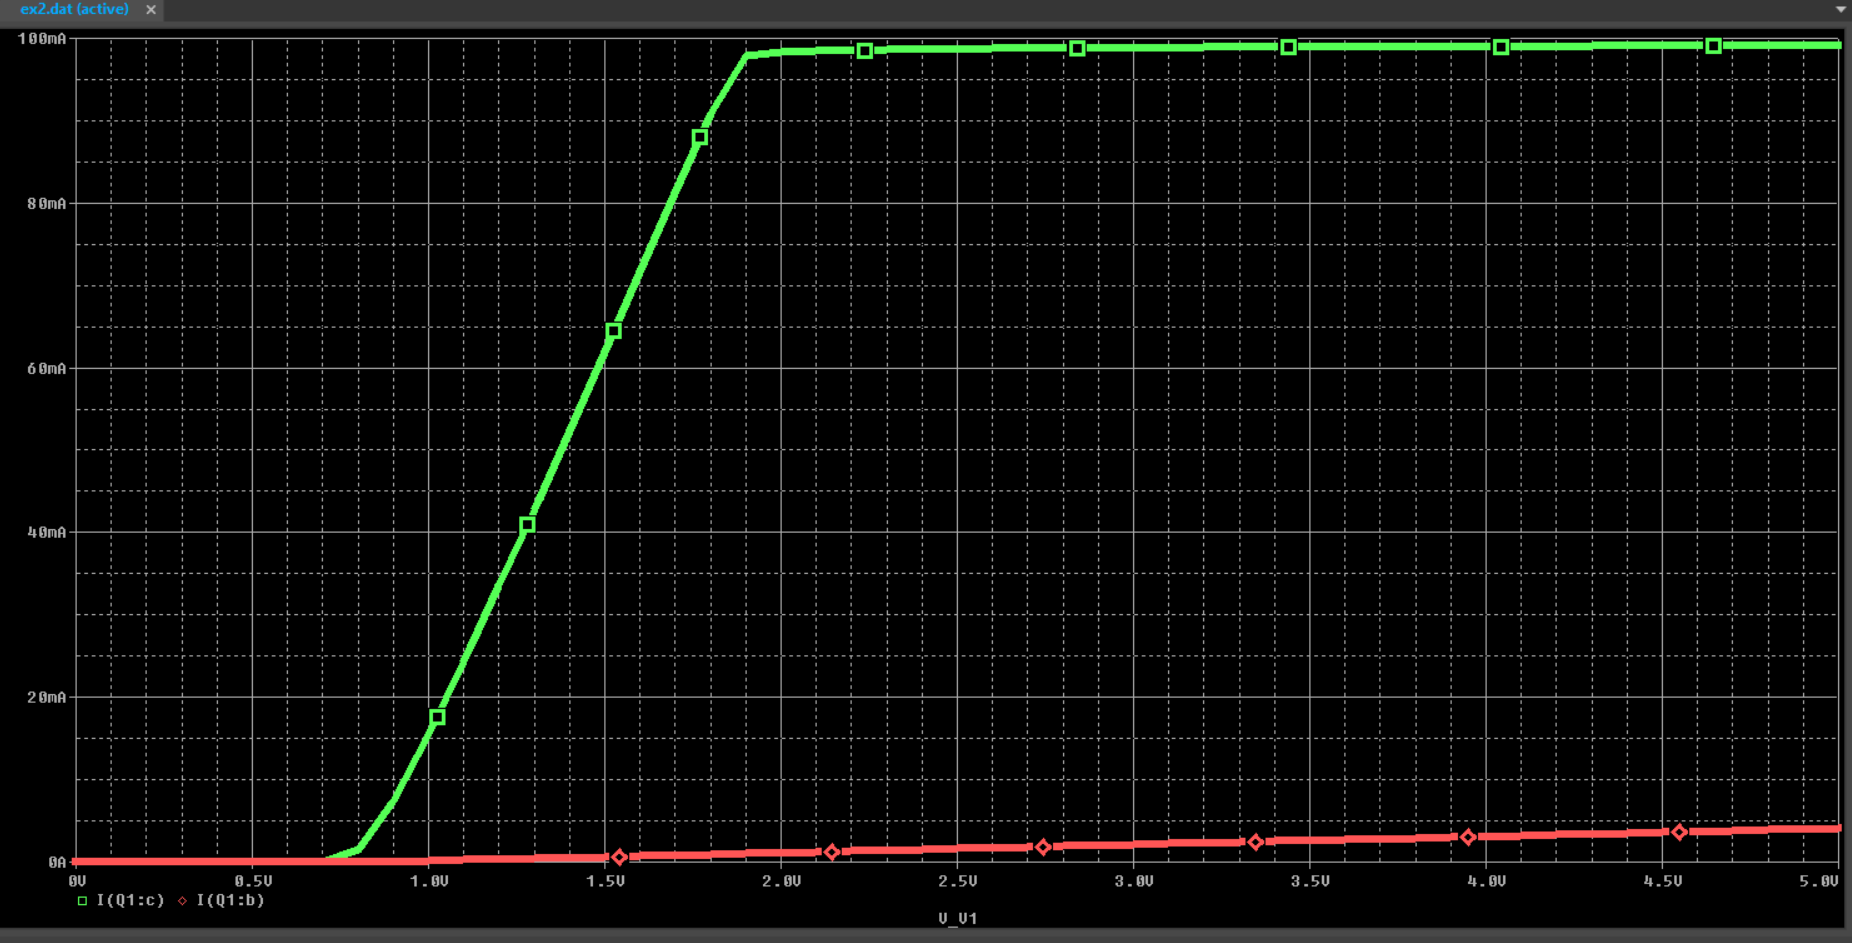
\includegraphics[width=1\linewidth]{graphics/ex2/f2.png}
    % \vspace{6cm}
\end{figure}

Khi transistor ở vùng bão hòa, giá trị \( V_1 \approx 1.9\) V.  

Lúc này, giá trị $I_B \approx  1 $ mA ; và giá trị $I_{C(Sat)} \approx 98 $ mA.